\chapter{Construction d'un Générateur de Portefeuilles de Passifs Réaliste}

\section{Objectifs Stratégiques et Contraintes Techniques}
La capacité à tester la robustesse des modèles et la pertinence des analyses de sensibilité repose sur un prérequis fondamental : la disponibilité de données de passif variées et réalistes. Pour un cabinet de conseil, où l'accès aux portefeuilles des clients n'est pas systématique, la faculté de générer des portefeuilles synthétiques, mais représentatifs du marché, constitue un atout stratégique majeur. C'est dans ce contexte qu'un générateur de portefeuilles de passifs a été conçu et développé dans le cadre de ce mémoire.

Ce chapitre a pour vocation de présenter cet outil essentiel. Nous détaillerons les besoins stratégiques et analytiques auxquels il répond, la méthodologie de génération retenue, les contraintes techniques rencontrées et les données qui ont été utilisées pour rendre le portefeuille le plus réaliste possible.

 
\subsection{Définition du générateur de portefeuilles de passifs}
Un générateur de portefeuille de passifs est un outil conçu pour créer, de manière algorithmique, des ensembles de données synthétiques qui imitent avec réalisme des portefeuilles de contrats d'assurance-vie. Plutôt que de s'appuyer sur des données réelles, souvent confidentielles ou indisponibles, cet outil simule les caractéristiques fondamentales des assurés (âge, sexe, etc.) et de leurs contrats (type de produit, montant de la provision mathématique, date de souscription, etc.).

L'objectif n'est pas de produire des données aléatoires, mais de générer un portefeuille dont les propriétés statistiques — distributions, corrélations, tendances — sont indiscernables de celles d'un portefeuille réel. Il s'agit d'une brique essentielle pour l'analyse quantitative en actuariat, permettant de surmonter les contraintes d'accès aux données. Le développement d'un tel outil s'est imposé comme une nécessité pour plusieurs raisons stratégiques et analytiques.


\subsection{Besoins métiers : simulation de nouveaux produits et analyse concurrentielle}
Pour un acteur du secteur de l'assurance, qu'il s'agisse d'un assureur ou d'un cabinet de conseil, la capacité à modéliser et à anticiper les dynamiques de marché est un avantage concurrentiel décisif. Le générateur de portefeuilles de passifs répond directement à ce besoin en fournissant un support quantitatif pour la prise de décision stratégique. Il permet par exemple à un cabinet de conseil de tester ses modèles sans dépendre des données clients, et à un assureur d'explorer des scénarios prospectifs ou d'évaluer l'impact de nouvelles offres. Son utilité se manifeste dans trois domaines clés pour les assureurs : le lancement de nouveaux produits, l'orientation du \textit{business mix} et l'analyse concurrentielle.

Premièrement, le lancement d'un nouveau produit d'assurance-vie représente un investissement et un risque significatifs. Avant toute commercialisation, il est impératif d'en évaluer rigoureusement les impacts sur le profil de risque et la rentabilité de l'entreprise. Le générateur offre un véritable laboratoire virtuel pour effectuer ces tests. En simulant l'intégration de milliers de polices conformes aux caractéristiques du nouveau produit (garanties, frais, options), il permet de projeter leur comportement dans le temps. Il devient alors possible d'analyser leur effet sur les indicateurs prudentiels de Solvabilité II, tels que le \textit{Best Estimate} (BE) et le \textit{Solvency Capital Requirement} (SCR), mais aussi d'évaluer leur sensibilité à divers chocs de marché (hausse des taux, krach boursier) ou de comportement (vagues de rachats). Cet outil permet ainsi de tester, d'ajuster et d'optimiser les caractéristiques d'un produit pour atteindre le couple rendement/risque désiré avant même sa mise sur le marché.

Deuxièmement, le générateur est un outil précieux pour piloter la stratégie à long terme de l'entreprise. La direction peut être amenée à vouloir faire évoluer son \textit{business mix}, c'est-à-dire la répartition de son portefeuille entre différents types de produits (fonds en euros, unités de compte, prévoyance...). Par exemple, dans un contexte de taux bas persistants, un assureur pourrait vouloir accélérer sa transition vers les produits en unités de compte. Le générateur permet de quantifier les implications d'une telle stratégie. En simulant des portefeuilles futurs correspondant à ces nouvelles orientations commerciales, la direction peut visualiser les conséquences sur le bilan, la rentabilité prévisionnelle, mais aussi sur la consommation de capital et l'exposition aux risques. Ces simulations éclairent les décisions stratégiques et s'intègrent naturellement dans des exercices prospectifs comme l'ORSA (\textit{Own Risk and Solvency Assessment}).

Enfin, la capacité à se positionner par rapport à ses concurrents est fondamentale. Faute d'accès aux portefeuilles détaillés des autres acteurs, un assureur doit s'appuyer sur des reconstitutions. En se basant sur des données publiques (rapports annuels ou publications réglementaires comme les SFCR) ou des statistiques sectorielles, le générateur peut permettre la création d'un portefeuille représentatif du marché, ou simuler le portefeuille probable d'un concurrent spécifique. Ces portefeuilles synthétiques deviennent alors une base solide pour des analyses comparatives (\textit{benchmarking}). Ils permettent non seulement d'évaluer la performance relative, mais aussi de comparer les profils de risque, d'anticiper les stratégies concurrentes et d'identifier les meilleures pratiques du marché. Il convient toutefois de souligner les limites d'une telle démarche. Une analyse ALM complète et réaliste d'un concurrent ne peut se contenter de la seule modélisation du passif. Elle exigerait également de simuler son portefeuille d'actifs et de disposer d'informations précises sur ses ressources financières et ses fonds propres. Or, ces données, qui relèvent du secret des affaires, sont rarement publiques. Par conséquent, l'analyse comparative reste nécessairement partielle, se concentrant sur les caractéristiques intrinsèques du portefeuille de passifs reconstitué.
\bigskip

\begin{figure}[h!]
    \centering
    \begin{tikzpicture}[
        node distance=1ex,
        box/.style={
            rectangle,
            rounded corners=4pt,
            draw=gray,
            fill=white,
            very thin,
            inner sep=15pt,
            minimum width=3cm,
            minimum height=2cm,
            align=center,
            font=\sffamily\bfseries\color{black}
        },
        arrow/.style={
            -Latex,
            very thin,
            color=accenture,
            line width=2pt
        }
    ]

    % Nodes
    \node[box] (input) {Données d'entrée :\\- Rapports d'assureurs\\- Marché français};
    \node[box, right=4ex of input] (process) {Modélisation et calibrage :\\- Distributions\\- Corrélations};
    \node[box, right=4ex of process] (output) {Portefeuille synthétique};

    % Arrows
    \draw [arrow] (input) -- (process);
    \draw [arrow] (process) -- (output);

    \end{tikzpicture}
    \caption{Schéma de la méthodologie de génération d'un portefeuille de passifs synthétique.}
    \label{fig:methodologie_horizontale}
\end{figure}

\subsection{Défis de la modélisation : réalisme, volumétrie et flexibilité}

La conception et la mise en œuvre d'un générateur de portefeuilles de passifs efficace soulèvent trois défis majeurs et interdépendants :

\begin{itemize}
\item \textbf{Le réalisme des données générées :} Il s'agit du défi le plus fondamental. L'objectif n'est pas de produire des données aléatoires, mais de créer un portefeuille synthétique dont les propriétés statistiques sont indiscernables de celles d'un portefeuille réel. Cela implique non seulement de reproduire fidèlement les distributions de chaque caractéristique individuelle (âge, montant, etc.), mais aussi, et surtout, de capturer les corrélations complexes qui les lient. Par exemple, l'âge d'un assuré est souvent corrélé au type de produit souscrit et au montant de sa provision mathématique. Ignorer ces dépendances conduirait à un portefeuille incohérent, dont le comportement sous différents scénarios de risque serait erroné, invalidant ainsi les analyses prudentielles ou stratégiques qui en découlent.

\item \textbf{La gestion de la volumétrie :} Les portefeuilles d'assurance-vie des grands acteurs du marché se comptent en centaines de milliers, voire en millions de contrats. Le générateur doit être capable de produire des ensembles de données de cette ampleur de manière performante, c'est-à-dire dans un temps de calcul raisonnable et sans consommer une quantité prohibitive de ressources mémoire. Cette contrainte de performance est d'autant plus forte que la gestion des corrélations, nécessaire au réalisme du portefeuille, ajoute une complexité de calcul significative. Il faut donc trouver un équilibre entre la sophistication statistique et la performance, ce qui a des implications directes sur les choix technologiques et algorithmiques.

\item \textbf{La flexibilité de l'outil :} Un générateur ne serait que d'une utilité limitée s'il ne produisait qu'un seul type de portefeuille statique. Pour répondre aux besoins métiers variés, l'outil doit être hautement paramétrable. L'utilisateur doit pouvoir ajuster finement les caractéristiques du portefeuille à générer : définir les spécificités d'un nouveau produit, modifier les distributions statistiques pour simuler un segment de marché différent, ou encore changer les lois de comportement (rachat, mortalité) pour tester de nouvelles hypothèses. Cette flexibilité est la clé qui transforme le générateur en un véritable laboratoire d'expérimentation pour les actuaires et les stratèges.
\end{itemize}

Relever ces trois défis a nécessité de concevoir une architecture alliant rigueur statistique et performance calculatoire. La section suivante présente en détail la méthodologie de modélisation probabiliste qui a été développée pour construire un portefeuille à la fois réaliste, volumineux et flexible.

\section{Méthodologie de Génération et Modélisation Statistique}

La méthodologie de génération du portefeuille de passifs synthétique repose sur une approche probabiliste. L'objectif est de construire un ensemble de contrats d'assurance dont les propriétés statistiques sont entièrement maîtrisées. Pour ce faire, chaque caractéristique d'un contrat (âge de l'assuré, montant de la provision, etc.) est modélisée comme une variable aléatoire, tirée d'une loi de probabilité préalablement calibrée sur des données de marché quand elles sont disponibles. Sinon, des hypothèses ont été formulées pour recréer ces variables de la manière la plus réaliste possible.


\subsection{Approche stochastique par lois de probabilité}

La génération du portefeuille synthétique s'appuie sur une modélisation stochastique où chaque attribut d'un contrat est représenté par une variable aléatoire. Dans un premier temps, l'objectif est de générer un portefeuille complet, représentatif du marché. Pour ce faire, une loi de probabilité marginale est définie pour chaque caractéristique, avec des paramètres rigoureusement calibrés sur des données de marché. Certaines variables sont ensuite liées entre elles pour refléter les dépendances observées dans les portefeuilles réels. Ce même cadre peut ensuite être adapté pour simuler un produit spécifique ; il suffirait alors de générer des variables aléatoires de manière conditionnelle aux caractéristiques de ce produit. Cette méthode garantit à la fois le réalisme statistique du portefeuille et la flexibilité nécessaire aux analyses prospectives.

Les sections suivantes détailleront la méthodologie de calibration pour les variables fondamentales qui structurent le portefeuille :
\begin{itemize}
    \item L'âge de l'assuré ;
    \item L'âge à la souscription, qui détermine l'ancienneté du contrat ;
    \item Le montant de la Provision Mathématique (PM).
\end{itemize}
D'autres variables, telles que le sexe ou la répartition des supports, seront également modélisées pour compléter le profil de chaque contrat.


\subsubsection{Modélisation de l'âge des assurés}

La première étape a consisté à construire une distribution de probabilité réaliste à partir de deux sources de données :
\begin{enumerate}
\item \textbf{La pyramide des âges de la population française} pour l'année 2024 \cite{pyramide_age}, fournissant la structure démographique de base entre 0 et 100 ans.

\item \textbf{Une étude statistique de l'INSEE} sur la détention d'assurance-vie par tranche d'âge en France \cite{insee_prop_av_age}
\begin{figure}[H]
\centering
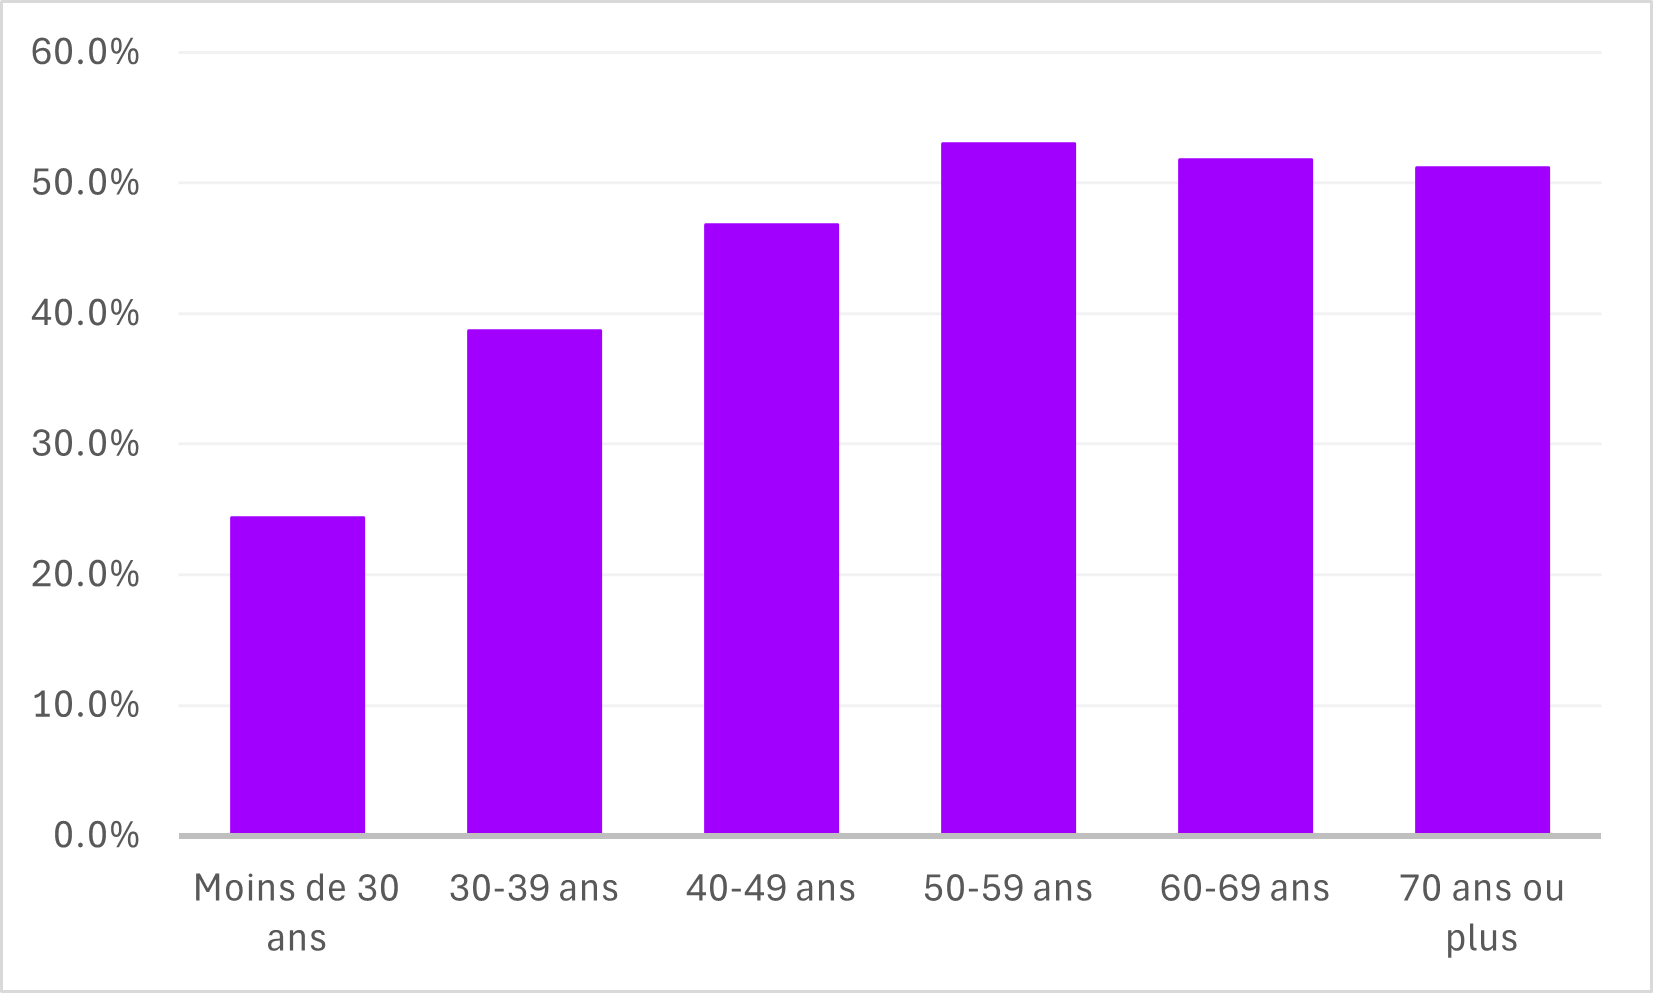
\includegraphics[width=0.7\textwidth]{images/2_chapitres/chapitre3/insee_prop_av_age.png}
\caption{Proportion de détention d'assurance-vie par tranche d'âge en France \cite{insee_prop_av_age}.}
\label{fig:insee_prop_av_age}
\end{figure}
\end{enumerate}
Afin de transformer les données discrètes de l'INSEE, présentées par tranches d'âge, en une distribution continue du taux de détention par âge, une méthodologie d'interpolation a été mise en œuvre. Cette étape est cruciale pour pouvoir ensuite simuler l'âge des assurés de manière réaliste.

L'approche a consisté à définir d'abord des points de données représentatifs pour chaque tranche d'âge fournie. Pour les tranches intermédiaires (par exemple, 30-39 ans), le point central de l'intervalle a été retenu. Pour les tranches extrêmes, des hypothèses spécifiques ont été formulées :
\begin{itemize}
    \item Pour la tranche des moins de 30 ans, plusieurs points ont été positionnés entre 18 et 30 ans afin de modéliser la croissance progressive de la détention en début de vie active.
    \item Pour la tranche des "70 ans et plus", un âge représentatif de 82,5 ans a été choisi.
\end{itemize}

Une fois ces points définis, une interpolation cubique par morceaux préservant la monotonie (PCHIP, \textit{Piecewise Cubic Hermite Interpolating Polynomial}) a été appliquée sur la majeure partie de la courbe. Cette méthode a été privilégiée car elle évite les oscillations artificielles et garantit que la proportion de détention reste croissante là où les données le suggèrent. Pour les âges plus avancés, une interpolation linéaire a été utilisée pour assurer une transition douce, suivie d'un plateau constant après 82,5 ans. Cette dernière hypothèse modélise une stabilisation du comportement de détention chez les assurés les plus âgés avec une absence de rachats.

Le résultat de ce processus est une fonction continue et lisse qui estime le taux de détention d'assurance-vie pour chaque âge entre 18 et 100 ans, comme illustré par la figure \ref{fig:interpolation_prop_age}.

\begin{figure}[H]
\centering
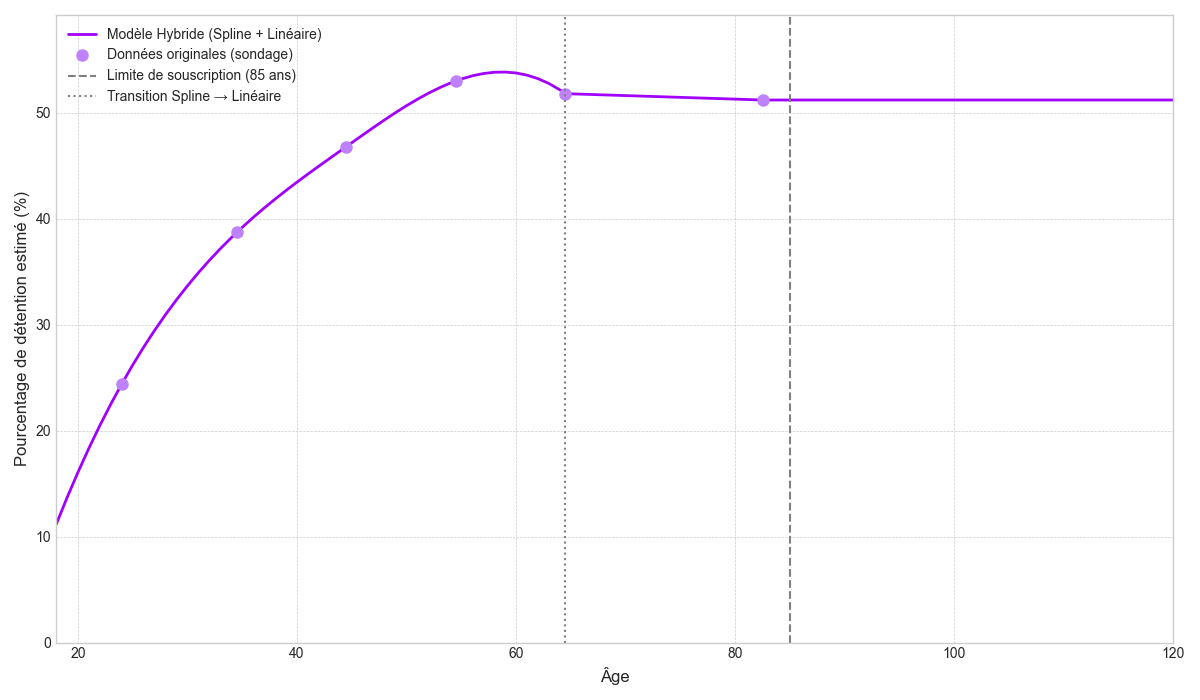
\includegraphics[width=0.7\textwidth]{images/2_chapitres/chapitre3/interpolation_prop_age.png}
\caption{Proportion de détention d'assurance-vie par âge en France par diverses méthodes d'interpolation.}
\label{fig:interpolation_prop_age}
\end{figure}


En multipliant la population de chaque âge par le taux de détention estimé, il a été possible d'obtenir une estimation du nombre d'assurés pour chaque âge et chaque sexe. Après normalisation, il est désormais possible de construire une loi de probabilité empirique. Ensuite deux lois de probabilité continues ont été sélectionnées comme candidates pour modéliser la distribution empirique : la \textbf{loi Gamma} et la \textbf{loi Beta}. Les paramètres de ces deux lois ont été estimés par la méthode du maximum de vraisemblance sur un échantillon de 200 000 individus tirés de la loi empirique. Pour déterminer la loi la plus adéquate, des critères visuels et statistiques (Test de Kolmogorov-Smirnov, AIC, BIC) ont été utilisés. La figure \ref{fig:beta} montre l'ajustement de la loi Beta qui a des meilleurs résultats statistiques et qui épouse mieux la distribution empirique que la loi Gamma (figure \ref{fig:gamma}). 

\begin{figure}[H]
\centering
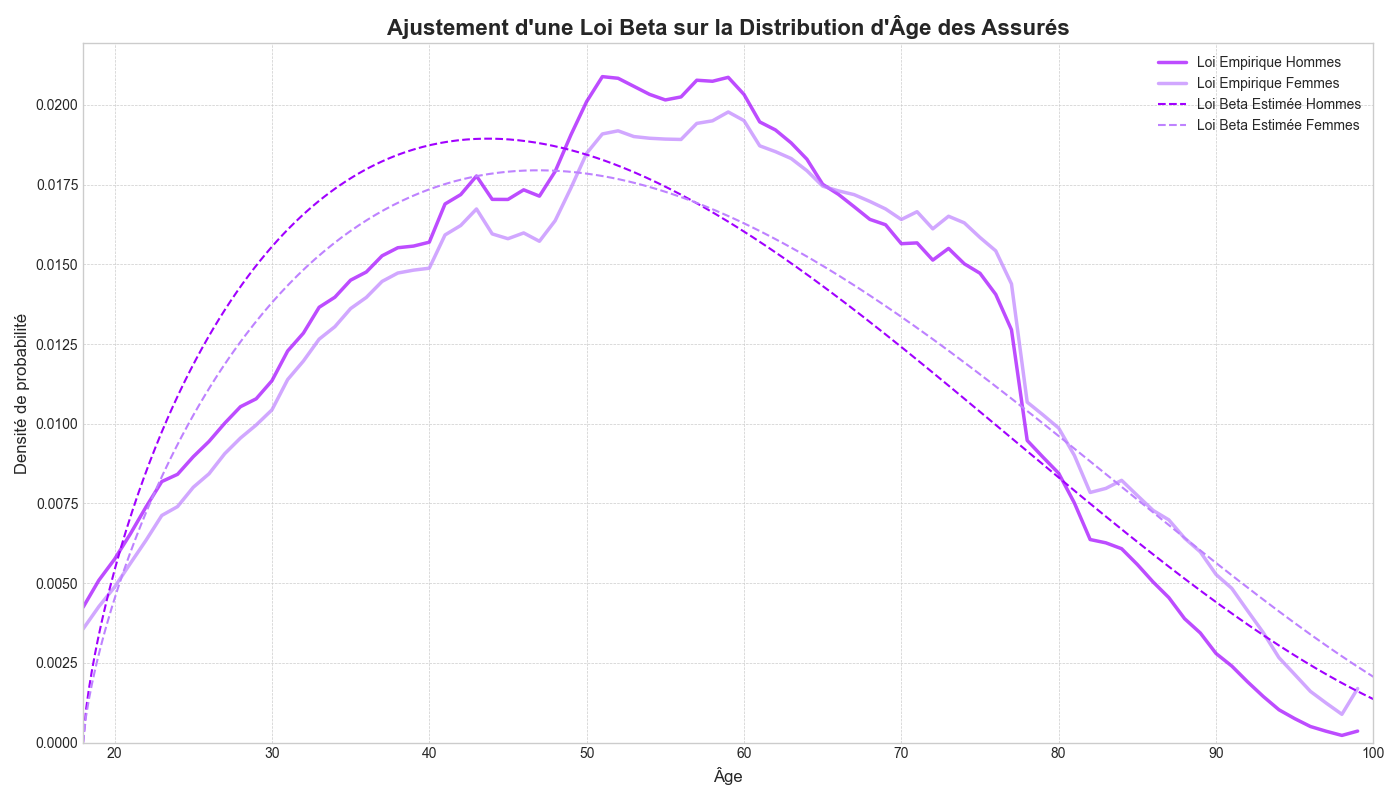
\includegraphics[width=0.8 \textwidth]{images/2_chapitres/chapitre3/estimation_loi_beta.png}
\caption{Ajustement de la loi Beta sur la distribution empirique.}
\label{fig:beta}
\end{figure}

Le tableau \ref{tab:stats} confirme cette observation. La loi Beta présente une statistique K-S deux fois plus faible et des scores AIC et BIC significativement inférieurs, indiquant un meilleur ajustement. C'est donc cette loi qui a été retenue pour modéliser l'âge des assurés dans le portefeuille synthétique.

\begin{table}[H]
\centering
\begin{tabular}{@{}lccc@{}}
\toprule
\textbf{Métrique} & \textbf{Loi Gamma} & \textbf{Loi Beta} & \textbf{Meilleur Modèle} \\
\midrule
Statistique K-S (D) & 0.0396 & 0.0271 & Beta \\
AIC (Akaike) & 1 674 497 & 1 668 357 & Beta \\
BIC (Bayésien) & 1 674 527 & 1 668 378 & Beta \\
\bottomrule
\end{tabular}
\caption{Tableau comparatif des métriques d'ajustement (population masculine).}
\label{tab:stats}
\end{table}

\subsubsection{Modélisation de l'âge à la souscription}
Une fois l'âge des assurés modélisé, il est indispensable de déterminer l'âge à la souscription. Cette variable est fondamentale, car elle permet de calculer l'ancienneté du contrat, un paramètre clé qui influence directement les lois de comportement, notamment les taux de rachat, dans les modèles de projection.

La distribution de l'âge à la souscription n'a pas été calibrée sur des données directes, mais a été dérivée de la courbe de taux de détention par âge, établie dans la section précédente. L'hypothèse sous-jacente est que la densité de probabilité de souscrire à un âge donné est proportionnelle à la vitesse à laquelle le taux de détention augmente à cet âge. Autrement dit, la distribution de l'âge à la souscription peut être approximée par la dérivée discrète de la fonction du taux de détention. Par exemple, une forte pente de la courbe de détention entre 25 et 35 ans signale une intense activité de souscription dans cette tranche d'âge. En calculant la différence finie entre les points de la courbe interpolée, il est donc possible de construire une distribution empirique de l'âge à la souscription.

\begin{figure}[H]
\centering
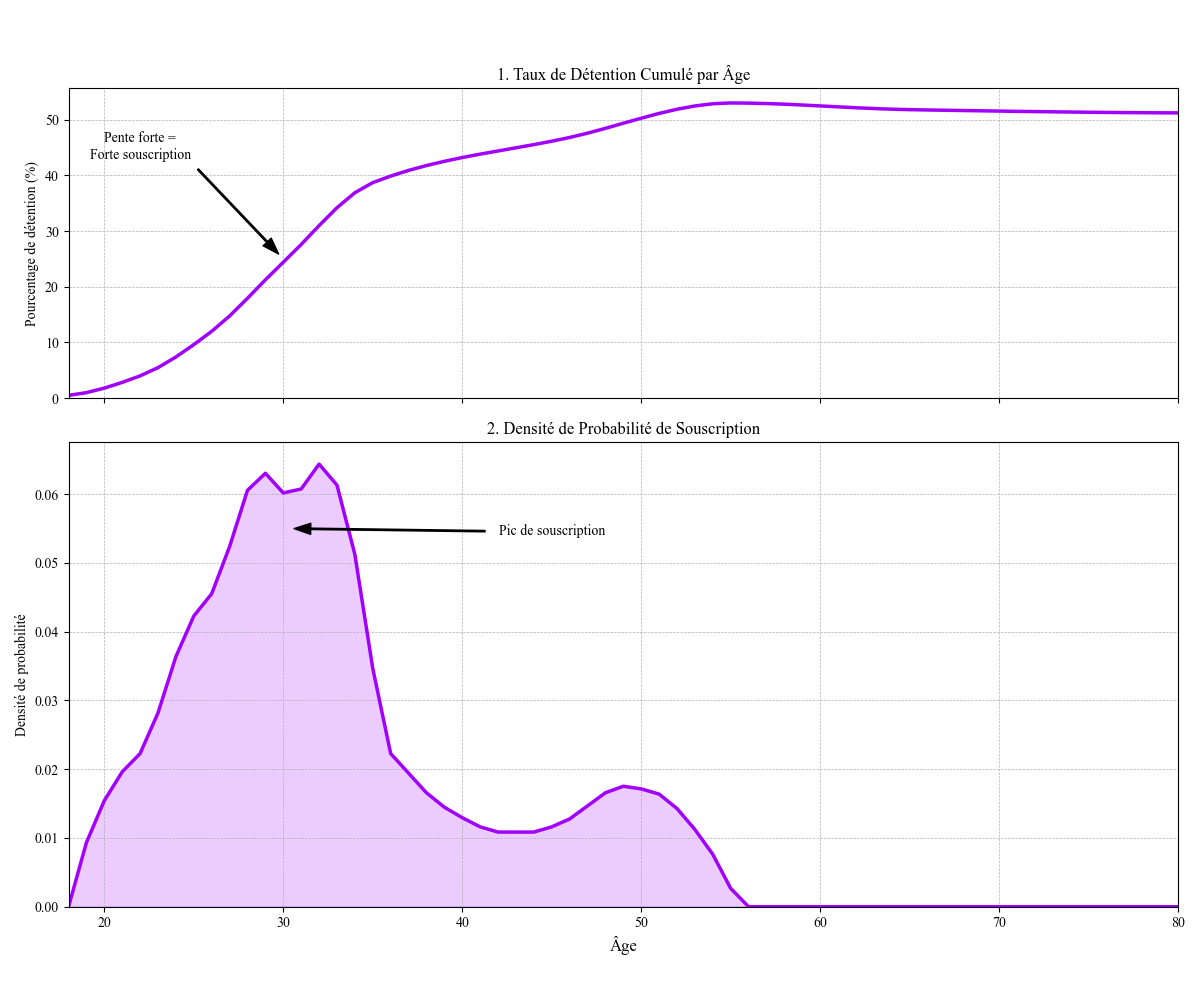
\includegraphics[width=0.9\textwidth]{images/2_chapitres/chapitre3/derivation_dist_souscription.png}
\caption{Passage de la distribution empirique de l'âge à la souscription à la densité de probabilité du taux de souscription.}

\end{figure}

Plusieurs lois de probabilité ont été testées pour modéliser cette distribution empirique de l'âge à la souscription : Gamma, Beta, Weibull, et un modèle de Mélange Gaussien (GMM). Le tableau \ref{tab:stats_souscription} présente les résultats.

\begin{table}[H]
\centering
\begin{tabular}{@{}lcccc@{}}
\toprule
\textbf{Distribution} & \textbf{AIC} & \textbf{BIC} & \textbf{K-S (D)} \\
\midrule
GMM (n=2) & 1 125 603 & 1 125 654 & 0.0485 \\
Beta & 1 385 454 & 1 385 495 & 0.0845 \\
Gamma & 1 400 178 & 1 400 208 & 0.1110 \\
Weibull & 1 437 176 & 1 437 207 & 0.1544 \\
\bottomrule
\end{tabular}
\caption{Tableau comparatif des métriques d'ajustement pour l'âge à la souscription.}
\label{tab:stats_souscription}
\end{table}

Le \textbf{Mélange Gaussien à deux composantes (GMM)} s'est avéré être le modèle le plus performant, avec des scores AIC et BIC nettement inférieurs. Cela s'explique car 2 pics de souscription sont observables sur la distribution. Cette bimodalité, illustrée par la calibration de la loi GMM en figure \ref{fig:gmm_souscription}, est une caractéristique de marché que les lois de probabilité plus simples ne peuvent capturer.

\begin{figure}[H]
\centering
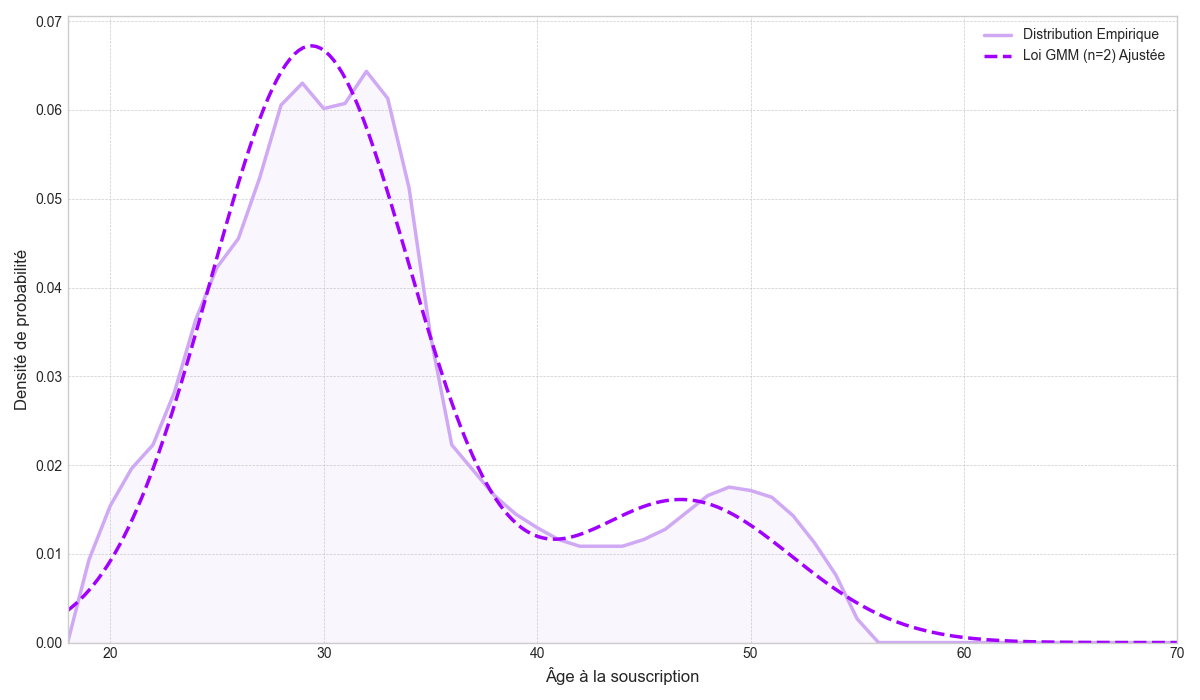
\includegraphics[width=0.9\textwidth]{images/2_chapitres/chapitre3/calibration_loi_GMM_souscription.png}
\caption{Ajustement d'une GMM sur la distribution de l'âge à la souscription.}
\label{fig:gmm_souscription}
\end{figure}


\subsubsection{Modélisation de la Provision Mathématique (PM)}

Pour calculer la Provision Mathématique à partir des données marché, une méthode plus complexe a été mise en place. Une approche directe consistant à ajuster une loi sur des données de PM n'est pas possible car des données publiques sur ce sujet n'existent pas. Une méthodologie de modélisation conditionnelle a donc été mise en place.

L'hypothèse fondamentale est que la PM d'un individu est principalement fonction de son \textbf{patrimoine}, qui lui-même est fortement corrélé à son \textbf{âge}. La modélisation s'est donc déroulée en plusieurs étapes.


La première étape a consisté à modéliser la distribution du patrimoine brut en fonction de l'âge, en s'appuyant sur les données de l'INSEE \cite{insee_patrimoine_age}. Plutôt que de calibrer une seule loi pour toute la population, une \textbf{loi Lognormale} a été ajustée pour chaque tranche d'âge. Les paramètres de cette loi, $\mu$ et $\sigma$, ont été estimés par la méthode de \textbf{correspondance des quantiles}, en s'assurant que la médiane et les déciles de la loi ajustée correspondent à ceux observés dans les données. Le tableau \ref{tab:params_patrimoine_age} synthétise les paramètres obtenus.

\begin{table}[H]
\centering
\begin{tabular}{@{}lccc@{}}
\toprule
\textbf{Tranche d'âge} & $\mu$ & $\sigma$ \\
\midrule
Moins de 30 ans & 9.9233 & 1.7713 \\
30 à 39 ans & 11.6750 & 1.8374 \\
40 à 49 ans & 12.1756 & 2.1221 \\
50 à 59 ans & 12.3216 & 2.0551 \\
60 à 69 ans & 12.3579 & 2.0772 \\
70 ans ou plus & 12.2620 & 1.8199 \\
\bottomrule
\end{tabular}
\caption{Paramètres de la loi Lognormale du patrimoine brut, calibrés par tranche d'âge.}
\label{tab:params_patrimoine_age}
\end{table}




Sur la base des calibrations précédentes, une population synthétique de 500 000 individus a été générée. Pour chaque individu, un âge a été tiré selon la loi Beta déterminée précédemment, puis un patrimoine a été tiré selon la loi Lognormale conditionnelle correspondant à son âge. On obtient ainsi un échantillon de paires (Âge, Patrimoine) respectant la corrélation observée dans la réalité.

La deuxième étape consiste à estimer la part du patrimoine de chaque individu allouée à l'assurance-vie. Pour ce faire, les données de l'INSEE sur la composition du patrimoine par décile \cite{insee_patrimoine_age} sont utilisées. La figure \ref{fig:composition_patrimoine} illustre la part du patrimoine financier en fonction du patrimoine brut moyen. Cette relation n'est pas linéaire. Pour les patrimoines les plus modestes, qui n'ont pas encore la capacité d'investir dans l'immobilier, la part des actifs financiers est relativement élevée. À mesure que le patrimoine augmente, une part significative est allouée à l'immobilier, ce qui diminue mécaniquement la part relative du patrimoine financier. Ce phénomène s'inverse cependant pour les patrimoines les plus élevés, où la diversification vers des actifs financiers redevient prépondérante, entraînant une remontée de leur part dans le patrimoine total, ce n'est pas observable sur le graphique \ref{fig:composition_patrimoine} car les données sont agrégées par décile.

\begin{figure}[H]
    \centering
    \begin{tikzpicture}
        \begin{axis}[
            xlabel={Patrimoine brut moyen (€)},
            ylabel={Patrimoine financier (\%)},
            xmode=log,
            log ticks with fixed point,
            xticklabel style={
                /pgf/number format/fixed,
                /pgf/number format/precision=0,
                /pgf/number format/1000 sep={\,}
            },
            yticklabel style={
                /pgf/number format/fixed,
                /pgf/number format/precision=0
            },
            grid=major,
            width=\textwidth,
            height=8cm,
            legend pos=outer north east
        ]
        \addplot[
            smooth,
            mark=*,
            accenture,
        ] coordinates {
            (1900, 31.4)
            (8300, 33.9)
            (21500, 41.7)
            (64300, 43.0)
            (142100, 20.0)
            (211500, 14.4)
            (285900, 14.7)
            (383300, 16.4)
            (559800, 20.2)
            (1487700, 23.2)
        };
        \legend{Part du patrimoine financier}
        \end{axis}
    \end{tikzpicture}
    \caption{Part du patrimoine financier en fonction du patrimoine brut moyen, par décile \cite{insee_patrimoine_age}.}
    \label{fig:composition_patrimoine}
\end{figure}

La troisième étape consiste à lier le patrimoine financier à la Provision Mathématique. Il est en effet plus réaliste de considérer que l'épargne en assurance-vie (ou la provision mathématique du point de vue de l'assureur) constitue une part du patrimoine financier plutôt que du patrimoine brut. Une hypothèse centrale est donc formulée : la PM d'un individu est estimée comme une fraction de son patrimoine financier. Sur la base de données INSEE, cette fraction est fixée à \textbf{40\%}. Ainsi, pour chaque individu de la population simulée, la PM est calculée comme suit :
$$ \text{PM} = \text{Patrimoine Brut} \times \text{Part du Patrimoine Financier} \times 40\% $$
Cette règle permet de transformer la distribution de patrimoine en une distribution de PM, en tenant compte des non-linéarités observées dans la composition du patrimoine.

Après avoir appliqué ce processus à toute la population simulée, nous obtenons un échantillon réaliste de Provisions Mathématiques. Une dernière calibration a montré que la distribution de ces PM pouvait être modélisée de manière très satisfaisante par une \textbf{loi Lognormale}, comme l'indique le tableau \ref{tab:stats_pm}.

\begin{table}[H]
\centering
\begin{tabular}{@{}lccc@{}}
\toprule
\textbf{Distribution} & \textbf{AIC} & \textbf{BIC} & \textbf{K-S (D)} \\
\midrule
Lognorm & 7 142 088 & 7 142 120 & 0.017 \\
Gamma & 7 254 743 & 7 254 774 & 0.145 \\
\bottomrule
\end{tabular}
\caption{Pour le critère de Kolmogorov-Smirnov, la loi Lognormale est largement meilleure que la loi Gamma pour estimer cette distribution.}
\label{tab:stats_pm}
\end{table}


\subsection{Synthèse et Génération du Portefeuille Final}

Avec toutes les distributions marginales et conditionnelles calibrées, l'étape finale consiste à les assembler pour générer le portefeuille complet. Une approche par copule classique, où les trois variables (Âge, Âge Souscription, PM) seraient mises dans une copule 3D, a été écartée. Une telle approche simplifierait à l'excès les dépendances, en les réduisant à de simples coefficients de corrélation, et ne saurait capturer la richesse des relations non-linéaires (notamment l'évolution du patrimoine avec l'âge).

Un \textbf{modèle de génération hybride} a donc été privilégié :

\begin{enumerate}
    \item \textbf{Génération des âges par copule :} Une copule Gaussienne 2D est utilisée pour générer des paires corrélées (Âge de l'assuré, Âge de souscription), en utilisant les lois marginales calibrées (Gamma et GMM). Une contrainte assure que l'âge de souscription est toujours inférieur à l'âge de l'assuré.
    
    \item \textbf{Génération conditionnelle de la PM :} Pour chaque couple d'âges généré, la cascade de simulation décrite dans la section précédente est appliquée :
    \begin{itemize}
        \item On génère un patrimoine à partir de la loi Lognormale correspondant à l'âge de l'assuré.
        \item On simule la détention d'un contrat en fonction de ce patrimoine.
        \item Si un contrat est détenu, on calcule la PM en se basant sur la part de patrimoine financier et la règle des 40\%.
    \end{itemize}
\end{enumerate}

Ce processus itératif est répété jusqu'à obtenir le nombre de contrats désiré dans le portefeuille final. Le résultat est un fichier de données synthétique contenant trois variables dont les distributions et les interdépendances sont le reflet fidèle des analyses statistiques menées en amont. Cet outil fournit ainsi une base de données robuste et réaliste pour toutes les analyses actuarielles ultérieures.

A ce portefeuille synthétique de base, d'autres variables sont ajoutées pour enrichir le profil de chaque contrat. Ces variables supplémentaires sont également générées selon des lois de probabilité calibrées, comme résumé ci-dessous :

\begin{itemize}
    \item \textbf{Sexe de l'assuré :} Modélisé par une loi de Bernoulli $\mathcal{B}(p)$, où le paramètre $p$ représente la probabilité que l'assuré soit un homme. Ce paramètre est calibré à partir de statistiques démographiques publiques sur les détenteurs d'assurance-vie en France (INSEE), afin de refléter la répartition observée sur le marché.

    \item \textbf{Répartition de la PM entre fonds euros et unités de compte (UC) :} La part de la PM allouée aux UC est modélisée par une loi Bêta $\mathcal{B}eta(\alpha, \beta)$, dont les paramètres sont calibrés pour correspondre à la moyenne et à la variance de la répartition cible du portefeuille. La loi Bêta a été préférée à une loi Normale tronquée car son support naturel est l'intervalle $[0, 1]$, ce qui garantit la génération de proportions valides sans nécessiter de troncature ou de normalisation \textit{a posteriori}. La part allouée au fonds euros est ensuite déterminée comme le complément à 1.

    \item \textbf{Allocation d'actifs cible pour les UC :} Pour modéliser la répartition des actifs au sein des UC (actions, obligations, immobilier, etc.), une loi de Dirichlet $\text{Dir}(\boldsymbol{\alpha})$ est utilisée. Cette distribution est la généralisation multivariée de la loi Bêta et est spécifiquement conçue pour générer des vecteurs de nombres aléatoires qui respectent la contrainte de somme à 1 ($\sum_{i} \omega_i = 1$). Le vecteur de paramètres $\boldsymbol{\alpha} = (\alpha_1, \dots, \alpha_K)$ est calibré pour que l'espérance de chaque poids corresponde à l'allocation stratégique cible du produit. Cette approche est plus rigoureuse qu'une génération par lois Normales indépendantes suivie d'une normalisation, car elle préserve la structure de dépendance souhaitée entre les allocations.

    \item \textbf{Taux Minimum Garanti (TMG) :} Le TMG des contrats en modélisé en suivant l'année de souscription du contrat. En effet, les TMG ont tendance à diminuer avec le temps en raison de la baisse des taux d'intérêt, et cette relation temporelle est cruciale à capturer pour représenter fidèlement les risques associés aux contrats. Il a donc été décidé de modéliser le TMG de manière déterministe. Pour chaque année de souscription, une valeur de TMG est assignée en fonction des tendances historiques du marché. Par exemple, les contrats souscrits avant 2000 peuvent avoir un TMG de 3\%, ceux entre 2000 et 2010 un TMG de 2\%, ceux entre 2010 et 2020 un TMG de 1\%, et ceux après 2020 un TMG de 0\%. Cette approche garantit que le portefeuille synthétique reflète les conditions économiques réelles au moment de la souscription.
\end{itemize}

\section{Présentation de l'Outil et du Portefeuille de Référence Généré}
\subsection{Architecture de l'application en Python et choix technologiques}
% Votre texte ici...
\subsection{Description des paramètres d'entrée et des formats de sortie}
% Votre texte ici...
\subsection{Analyse descriptive du portefeuille de référence}
% Votre texte ici...


% \subsection{Description des contraintes techniques rencontrées}

% La conception du générateur a soulevé plusieurs contraintes techniques. La première fut de garantir le réalisme des portefeuilles générés. Il ne s'agit pas simplement de créer des données aléatoires, mais de reproduire les corrélations observées dans la réalité (par exemple, entre l'âge de l'assuré et le montant des primes). Une autre contrainte était liée à la volumétrie : l'outil devait être capable de générer des portefeuilles de plusieurs millions de lignes de manière performante. Enfin, la flexibilité était un critère essentiel ; l'outil devait permettre de paramétrer finement les caractéristiques des produits à simuler et les lois de comportement (rachat, mortalité) associées.

% \subsection{Méthodologie de génération des portefeuilles}

% La méthodologie adoptée repose sur une approche stochastique. Pour chaque caractéristique clé d'un contrat (âge de l'assuré, montant de la provision mathématique, type de support, etc.), une loi de probabilité a été définie et calibrée à partir de données de marché. L'outil génère ensuite, ligne par ligne, des assurés virtuels en tirant aléatoirement des valeurs selon ces distributions. Pour modéliser les dépendances entre les variables, des techniques de copules ont été envisagées afin de garantir la cohérence et le réalisme des profils générés. Le résultat est un portefeuille granulaire, au contrat près, qui peut ensuite être agrégé en \textit{model points} pour être utilisé dans le modèle de projection ALM.

% \subsection{Présentation de l'outil développé}

% L'outil final se présente comme une application développée en Python, dotée d'une interface permettant à l'utilisateur de paramétrer la simulation. Les entrées principales sont :
% \begin{itemize}
% \item Les caractéristiques du ou des produits à simuler (type de garantie, chargements, etc.).
% \item Les paramètres des lois statistiques pour chaque variable (âge, sexe, montant, etc.).
% \item La taille du portefeuille souhaité.
% \item Les lois de comportement (tables de mortalité, formules de rachat).
% \end{itemize}
% En sortie, l'outil produit un fichier standardisé contenant le portefeuille de passifs généré, directement exploitable par le modèle ALM.

% \section{Choix technologiques et environnement de développement}

% Le passage de VBA à un écosystème Python n'est pas anodin ; il reflète une orientation stratégique vers des technologies plus modernes, ouvertes et performantes, mieux adaptées aux défis du "Big Data" et des calculs intensifs en actuariat.

% \subsection{Migration vers des technologies modernes}
% L'environnement Excel/VBA, bien que très répandu, montre ses limites face à la complexité et à la volumétrie des modèles ALM modernes. La migration vers Python a permis de s'affranchir des limitations de mémoire et de performance d'Excel, tout en bénéficiant d'un langage structuré favorisant la qualité du code, la modularité et les tests automatisés, ce qui est un gage de maintenabilité et de fiabilité à long terme.

% \subsection{Avantages d'un langage open-source}
% Le choix de Python, un langage \textit{open-source}, présente des avantages considérables. D'un point de vue financier, il élimine les coûts de licence associés à de nombreux logiciels propriétaires. Plus important encore, il donne accès à une communauté mondiale de développeurs et de scientifiques, qui contribuent à un écosystème de librairies extrêmement riche et en constante évolution. Cette effervescence garantit un accès permanent aux algorithmes et aux techniques les plus récents.

% \subsection{Utilisation d'un écosystème dynamique}
% Le projet s'est appuyé sur des librairies de pointe pour la manipulation de données et le calcul scientifique. En particulier, l'utilisation de la librairie \textit{Polars} (ou alternativement \textit{Pandas}), écrite en Rust, a permis d'atteindre des niveaux de performance très élevés pour le traitement de grands volumes de données, dépassant de loin les capacités des outils traditionnels. Le fait que ces outils soient mis à jour très fréquemment par la communauté garantit que le modèle bénéficie en permanence des dernières optimisations et fonctionnalités.
